
%\documentclass{elsart}               % The use of LaTeX2e is preferred.

\documentclass[twocolumn]{autart}    % Enable this line and disable the 
                                     % preceding line to obtain a two-column 
                                     % document whose style resembles the
                                     % printed Automatica style.


\usepackage{graphicx}          % Include this line if your 
                               % document contains figures,
%\usepackage[dvips]{epsfig}    % or this line, depending on which
                               % you prefer.

\usepackage{graphicx}
\usepackage[utf8]{inputenc}

%\usepackage[spanish]{babel}
\usepackage{geometry}


\usepackage{ntheorem,lipsum}

\theorembodyfont{\upshape}
\newtheorem{thm}{Teorema}[section]
\newtheorem{definition}{Definition}[section]
\newtheorem{obs}{Observación}[section]
\newtheorem{proposition}{Proposition}[section]
\newtheorem{example}{Ejemplo}[section]
\newtheorem{problem}{Problem}[section]
\newtheorem{hipo}{Hipotesís}[section]

\usepackage{bm}

\usepackage{amsmath}
\usepackage{amssymb}

\DeclareMathOperator*{\argmax}{arg\,max}
\DeclareMathOperator*{\argmin}{arg\,min}
\usepackage{hyperref}
\hypersetup{
    colorlinks=true,
    linkcolor=blue,
    filecolor=magenta,      
    urlcolor=cyan,
}


\numberwithin{equation}{section}


\usepackage[Algoritmo]{algorithm}

\usepackage{algpseudocode}
\usepackage{caption}
\usepackage{subcaption}

\begin{document}

\begin{frontmatter}
\runtitle{Selective Harmonic Elimination via Optimal Control}   % Running title for regular 
                                              % papers but only if the title  
                                              % is over 5 words. Running title 
                                              % is not shown in output.

\title{Selective Harmonic Elimination via Optimal Control} % Title, preferably not more 
                                                 % than 10 words.

\thanks[footnoteinfo]{This paper was not presented at any IFAC 
meeting.}

\author[FD,UD]{Umberto Biccari}\ead{umberto.biccari@deusto.es},    % Add the 
\author[UAM,FD]{Carlos Esteve}\ead{carlos.esteve@uam.es},               % e-mail address 
\author[UD]{Jes\'us Oroya}\ead{djoroya@deusto.es}  % (ead) as shown
\address[FD]{Chair of Computational Mathematics, Fundaci\'on Deusto, Avenida de las Universidades 24, 48007 Bilbao, Basque Country, Spain.}  %
\address[UD]{Universidad de Deusto, Avenida de las Universidades 24, 48007 Bilbao, Basque Country, Spain.}  %
\address[UAM]{Departamento de Matem\'aticas, Universidad Aut\'onoma de Madrid, 28049 Madrid, Spain.}  % Please supply                                              
          
\begin{keyword}                           % Five to ten keywords,  
Selective Harmonic Elimination; Finite Set Control, Piecewise Linear function.               % chosen from the IFAC 
\end{keyword}                             % keyword list or with the 
                                          % help of the Automatica 
                                          % keyword wizard


\begin{abstract}                          % Abstract of not more than 200 words.
El problema de \emph{Selective Harmonic Elimination pulse-width modulation}(SHE) es planteado como el problema de control óptimo, con el fin de encontrar soluciones de ondas escalón sin prefijar el número de ángulos de conmutación. De esta manera, la metodología de control óptimo es capaz de encontar la forma de onda óptima y de encontrar la localizaciones de los ángulos de conmutación, incluso sin prefijar el número de conmutaciones. Este es un nuevo enfoque para el problema SHE en concreto y para los sistemas de control con un conjunto finito de controles admisibles en general.

\end{abstract}

\end{frontmatter}


\begin{abstract}
    En este documento formularemos el problema de \emph{Selective Harmonic Elimination pulse-width modulation}(SHE-PWM) como el problema de control óptimo, con el fin de encontrar soluciones de ondas cuadradas sin prefijar el número de ángulos de conmunatación. Esta nueva perspectiva nos permite realizar un análisis sobre la continuidad de soluciones.
\end{abstract}
\tableofcontents

\section{Introducción} 

The \emph{Selective Harmonic Elimination} (SHE) problem is a modulation method that allows you to generate step signals\footnote{It should be noted that the step signals we are talking about are discontinuous functions defined in the interval $ [0,2 \pi] $ and that they can only take values in a small and finite set of values.}.
with a desired harmonic spectrum.
%
That is, given some Fourier coefficients, the SHE problem looks for the step waveform $ \{u (\tau) | \tau \in (0,2 \pi] \} $ whose Fourier coefficients are as required.
%
In general, half-wave symmetry, that is $ u (\tau + \pi) = - u (\tau) $, is required so in this work we will focus on this case.
%
In this context, if the waveform and number of switching are fixed, the problem SHE can be formulated as an optimization problem where the variables to be optimized are the switching locations.
%
Then we look for the switching locations that minimize the Euclidean distance between coefficients of the sought function and the given coefficients.
\newline 

%%%%%%%%%%%%%%%%%%%%%%%%%%%%
%
Although the problem SHE given a preset waveform is easily solvable, there are several difficulties in its application.
%
It is not possible to calculate the switching locations by means of a real-time optimization, which is why the solutions for different values of objective Fourier coefficients are pre-calculated.
%
When a non-precalculated solution is required, interpolations are carried out with the help of the other solutions to obtain it.
%
However, it is known that the space of solutions at the commutation angles is discontinuous with respect to a continuous variation of objective Fourier coefficients.
%
This is the reason why the interpolation of solutions is complex and sometimes impossible.
\newline
%%%%%%%%%%%%%%%%%%%%%%%%%%%%%%%%%%%%%%%%%%%%%%%%%%%%%%%%%%%

%
The nature of the appearance and fading of solutions through a continuous variation of the Fourier coefficients is unknown.
%
By calculating of the solutions it is known that the more switching locations are considered, the larger the continuous region of solutions.
%
This tells us that the number of switching locations required along a region of the solution space could change so that this formulation is not very flexible for a continuous description of the solutions.
\newline
%%%%%%%%%%%%%%%%%%%%%%%%%%%%%%%%%%%%%%%%%%%%%%%%%%%%%%%%%%%

%
In this document we will present the SHE problem as an optimal control problem, where the optimization variable is the signal $ u (\tau) $ defined in the entire interval $ [0,2 \pi) $.
%
Thus we will describe how in the problem of the Fourier coefficients of the function $ u (\tau) $ they can be seen as the final state of a system controlled by $ u (\tau) $.
%
So the optimization is performed among all the possible functions that satisfy $ | u (\tau) | <1 $ that can control the final state at the desired Fourier coefficients.
%
Then we will show how to design a control problem so that the solution is a step function.
%
Finally, we will show solutions to the SHE problem by formulating the optimal control, seeing how this methodology is versatile in the face of the variation in the number of commutations.%


\section{Mathematical formulation of SHE}\label{Section2}

This section is devoted to the mathematical formulation of the SHE problem. In what follows, we with the notation $\mathcal U$ we will always refer to a finite set of real numbers contained in the interval $[-1,1]$:
\begin{align}\label{eq:Udef}
	\mathcal U = \{u_\ell\}_{\ell=1}^L\subset [-1,1]
\end{align}
Our objective is to design a piece-wise constant function $u(\tau):[0,2\pi)\to\mathcal U$ such that some of its lower-order Fourier coefficients take specific values determined a priori. 

Due to the application in power converters, we will focus here on functions with \textit{half-wave symmetry}, i. e. 
\begin{align*}
	u(\tau + \pi) = -u(\tau)\quad \mbox{for all}\; \tau \in [0,\pi).
\end{align*}
In this way, $u$ is fully determined by its values in the interval $[0,\pi)$, and its Fourier series expansion only involves the odd terms taking the form
\begin{equation}
	u(\tau ) = \sum_{\underset{i\, odd}{i \in \mathbb{N}}} a_i \cos(i\tau)+ \sum_{\underset{j\, odd}{j \in \mathbb{N}}}  b_j \sin(j \tau), 
\end{equation}
where the coefficients $a_i$ and $b_j$ are given by
\begin{equation} \label{eq:an}
	\begin{aligned}
		a_i = \frac{2}{\pi} \int_0^\pi u(\tau ) \cos(i \tau)\,d\tau, 
		\\
		b_j = \frac{2}{\pi} \int_0^\pi u(\tau)  \sin(j \tau)\,d\tau.
	\end{aligned}
\end{equation}
We can then give a general formulation of the SHE problem as follows:
\newline
\begin{problem}[SHE]\label{SHEp}
Let $\mathcal{U}$ be defined as in \eqref{eq:Udef} and let $\mathcal{E} _a $ and $\mathcal{E} _b $ be two sets of odd numbers with cardinalities $|\mathcal{E}_a| = N_a $ and $ |\mathcal{E} _b| = N_b$, respectively. Given the vectors $\bm{a}_T \in \mathbb{R}^{N_a}$ and $\bm{b}_T \in \mathbb{R}^{N_b} $, we look for $u:\in [0,\pi)\to\mathcal{U}$ such that 
\begin{gather}
	\notag a_i = (\bm{a}_T)_i, \quad\textrm{ for all } i \in \mathcal{E}_a,
	\\
	\notag b_j = (\bm {b}_T)_j, \quad\textrm{ for all } j \in \mathcal{E}_b,
\end{gather}
with $\{a_i\}_{i\in\mathcal E_a}$ and $\{b_j\}_{j\in\mathcal E_b}$ given by \eqref{eq:an}.
\end{problem} 

Figure \ref{} shows an example of a function $u$ solution of the SHE problem. 

\begin{figure}
	\centering
	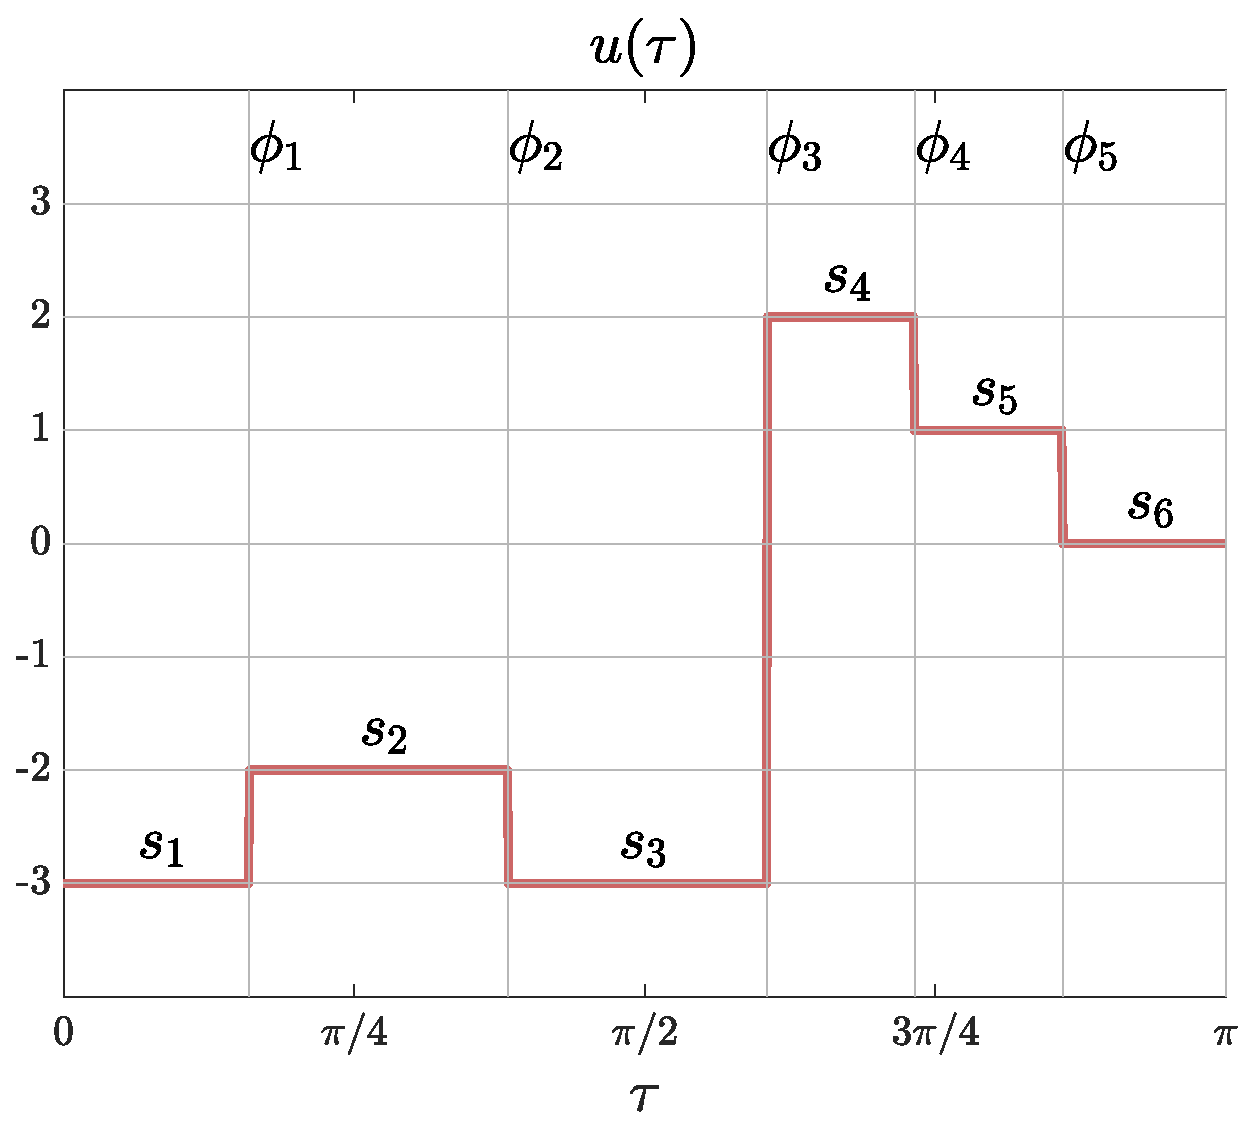
\includegraphics[scale=0.375]{img/fig01.eps} 
	\caption{Posible solution of problem \ref{SHEp}, where we consider that $\mathcal{U} = \{-3,\dots,3\}$}. We show the switching angles $\bm{\phi}$ and the waveform $\mathcal{S}$
\end{figure}
\textcolor{red}{Include here a picture of a possible solution $u$.}

As we anticipated in Section \ref{Section1}, the control signal $u$ is fully characterized by its waveform and the switching angles, to which we give a precise definition as follows:
\newline
\begin{definition}[Wave-form]\label{def:waveform}
Given a finite set of real numbers $\mathcal U$ defined as in \eqref{eq:Udef}, we will call a waveform any possible tuple $\mathcal S = (s_m)_{m=0}^{M+1}$ with $s_m\in \mathcal U$ for all $m=0,\ldots,M+1$.
\end{definition}
 
\begin{definition}[Switching angles]\label{def:switchingAngles}
Given a finite set of real numbers $\mathcal U$ defined as in \eqref{eq:Udef} and a piece-wise constant function $u:[0,\pi) \rightarrow \mathcal{U}$, we shall refer as switching angles $\bm{\phi} = \{\phi_m\}_{m=0}^{M+1}\subset[0,\pi]$, with $\phi_0 = 0$ and $\phi_{M+1} = \pi$, to the points in the domain $[0,\pi)$ where $u$ changes its value. 
\end{definition}

In view of the above definitions, we can provide the following explicit expression for the function $u$:
\begin{align}\label{eq:uExpl}
	&u = \sum_{m=0}^{M+1} s_m\chi_{[\phi_m,\phi_{m+1}]}
	\\
	&s_m\in\mathcal S, \;\phi_m\in{\bm{\phi}}, \quad \mbox{for all } m=0,\ldots,M+1, \notag 
\end{align}
where we denoted by $\chi_{[\phi_m,\phi_{m+1}]}$ the characteristic function of the interval $[\phi_m,\phi_{m+1}]$.

Besides, taking into account \eqref{eq:uExpl}, we can rewrite the Fourier coefficients \eqref{eq:an} as
\begin{align*}
	& a_i = a_i(\bm{\phi}) =  \frac{2}{i\pi} \sum_{k=1}^{M+1} s_k \Big[\sin(i\phi_k) -\sin(i\phi_{k-1})\Big]
	\\
	& b_j = b_j(\bm{\phi}) = \frac{2}{j\pi} \sum_{k=1}^{M+1} s_k \Big[\cos(j\phi_{k-1}) -\cos(j\phi_{k})\Big]
\end{align*}
Given a waveform $\mathcal S$, Problem \ref{SHEp} then reduces to find the switching locations $\bm{\phi}$ (see \cite{Yang2015,Konstantinou2010,Sun1996}). This can be cast as a minimization problem in the variables $\{\phi_m\}_{m=0}^{M+1}$, where the cost functional is the Euclidean distance between the obtained Fourier coefficients $\{a_i(\bm{\phi}),b_j(\bm{\phi})\}$ and the targets $(\bm{a},\bm{b})\in \mathbb{R}^{N_a}\times \mathbb{R}^{N_b}$.
\newline
\begin{problem}[Optimization for SHE]
Given a waveform $\mathcal S$ and a step function $u$ in the form \eqref{eq:uExpl}, we look for the switching angles $\bm{\phi}$ by means of the following minimization problem:
\begin{align}
	&\min_{\bm{\phi} \in [0,\pi]^{M}} \left(\sum_{i\in\mathcal{E}_a} \|a_T^i - a_i(\bm{\phi})\|^2 + \sum_{j\in \mathcal{E}_b} \|b_T^j - b_j(\bm{\phi})\|^2\right)\notag 
	\\[10pt]
	&\mbox{subject to: } 0 = \phi_0 <\phi_1 < \ldots < \phi_{M} < \phi_{M+1} = \pi \notag 
	\\
\end{align}
\end{problem}






Since the cardinality of $\mathcal S$ is not known a priori, meaning that we do not know how many switches will be necessary, it appears that the only solution to the SHE problem consists in fix the number of changes and counting all the possible combinations, to later solve an optimization problem for each one of them.
%
Taking into account that the number of possible multi-set $S$ is given by $|\mathcal{U}|^{|\mathcal S|}$, it is evident that the complexity of the above approach increases rapidly.
%
This problem has been studied in \cite{Yang2015} where, through appropriate algebraic transformations, the authors are able to convert the SHE problem into a polynomial system whose solutions' set contains all the possible waveforms for a given set $\mathcal{U}$ and number of elements in the sequence $\mathcal S$ which, however, is predetermined. 
%

On the other hand, we shall also mention that the SHE methodology has been developed to provide in real-time different target Fourier coefficients con with a $KHz$ latency. 
%
This makes impossible to find real-time solutions by optimization, making then necessary to pre-determine solutions that can later be interpolated.
%
Nevertheless, it is well-known that, fixed a sequence $S$, the continuity of the switching locations with respect to a continuous variation of the target Fourier coefficients may be quite cumbersome. 
%
In the majority of the cases, it is impossible to find a continuous solution in a large interval, an it is necessary to change the waveform $S$ while moving across different solution regions (\cite{Yang2015,Yang2017}). This makes difficult the interpolation of solutions and their finding.

In this document, we will present the SHE problem as an optimal control one, where the optimization variable is the signal $u(\tau)$ defined in the entire interval $[0,\pi)$. 
%
In particular, we will describe how the Fourier coefficients of the function $u(\tau)$ can be seen as the final state of a system controlled by $u (\tau)$. Hence, the optimization is performed among all the possible functions that satisfy $|u(\tau)|<1 $ and can control the final state at the desired Fourier coefficients. Then we will show how to design a control problem so that the solution is a step function.

In this way, we can reformulate Problem \ref{SHEp} as follows.
\newline
In this formulation, the SHE problem converts in a minimization problem with restrictions which can be solved by well-known techniques. Since the problem has several minimizers, we shall solve it employing global optimizers. Furthermore, since the choice of the waveform is arbitrary, we shall proceed in the same way for each possible waveform. 

{\color{red}{
    Tengo que enlazar estas sección con la formulacion de control óptimo.
}}
\section{SHE as a dynamical system}\label{Section3}

As we anticipated in Section \ref{Section1}, the main contribution of the present paper is to provide a novel and alternative approach to the SHE problem, based on optimal control. As we shall see, this methodology will allow us avoiding the choice of the waveform, as the optimization process selects the most convenient one in each case. 

To this end, the starting point is to rewrite the expression of the Fourier coefficients \eqref{eq:an} as the evolution of a dynamical system. This can be easily done by means of the fundamental theorem of differential calculus as follows: for all $i,j\in\mathbb{N}$, let $\alpha_i$ and $\beta_j$ be the solutions of the following Cauchy problems
\begin{align}\label{eq:Cauchy}
	\begin{cases} 
		\displaystyle\dot{\alpha_i}(\tau)  = \frac{2}{\pi}u(\tau)\cos(i\tau), & \tau\in [0,\pi) 
		\\[6pt]  
		\alpha_i(0)  = 0       
	\end{cases} \notag 
	\\
	\\
	\begin{cases} 
		\displaystyle\dot{\beta}_j(\tau)  = \frac{2}{\pi}u(\tau)\sin(j\tau), & \tau\in [0,\pi) 
		\\[6pt]  
		\beta_j(0) = 0       
	\end{cases}\notag
\end{align}
Then 
\begin{align*}
	&\alpha_i(\tau)= \frac{2}{\pi}\int_0^\tau u(\zeta) \cos(i\zeta)\,d\zeta 
	\\[5pt]
	&\beta_j(\tau) = \frac{2}{\pi}\int_0^\tau u(\zeta) \sin(j\zeta)\,d\zeta 
\end{align*}
and the Fourier coefficients \eqref{eq:an} are given by $a_i=\alpha_i(\pi)$ and $b_j=\beta_j(\pi)$.  

Let now
\begin{align*}
	\mathcal{E}_a = \{e_a^1,e_a^2,e_a^3,\dots,e_a^{N_a}\}, \quad \mathcal{E}_b = \{e_b^1,e_b^2,e_b^3,\dots,e_b^{N_b}\}    
\end{align*}
be two sets of odd numbers, and denote
\begin{align*}
	\bm{\alpha} = \{\alpha_i\}_{i\in\mathcal{E}_a}, \quad \bm{\beta} = \{\beta_j\}_{j\in\mathcal{E}_b}.
\end{align*}
Then, for any $\tau\in [0,\pi)$, we can define the vectors 
\begin{align*}
	\bm{\mathcal{D}}^\alpha(\tau) = 
	\begin{bmatrix} 
		\cos(e_a^1\tau) \\ \cos(e_a^2\tau) \\ \vdots \\ \cos(e_a^{N_a}\tau) 
	\end{bmatrix},
	\quad \bm{\mathcal{D}}^\beta(\tau) = 
	\begin{bmatrix} 
		\sin(e_b^1\tau) \\ \sin(e_b^2\tau) \\ \vdots \\ \sin(e_b^{N_b}\tau) 
	\end{bmatrix} 
\end{align*}
with $\bm{\mathcal{D}}^\beta(\tau) \in \mathbb{R}^{N_a} $ and $ \bm{\mathcal{D}}^\beta(\tau) \in \mathbb{R}^{N_b}$, and the dynamical systems \eqref{eq:Cauchy} can be rewritten in a vectorial form as:
\begin{align}\label{eq:CauchyVec}
	\begin{cases}
		\displaystyle \dot{\bm{\alpha}}(\tau) = \frac 2\pi \bm{\mathcal{D}}^\alpha(\tau) u(\tau), & \tau \in [0,\pi)
		\\[6pt]
		\bm{\alpha}(0) = 0
	\end{cases} \notag
	\\
	\\
	\begin{cases}
		\displaystyle\dot{\bm{\beta}}(\tau)  = \frac 2\pi \bm{\mathcal{D}}^\beta(\tau) u(\tau), & \tau \in [0,\pi) 
		\\[6pt]
		\bm{\beta}(0) = 0
	\end{cases}\notag 
\end{align}
Finally, compressing the notation even more, we can now denote 
\begin{align*}
	\bm{x}(\tau) = \begin{bmatrix} \bm{\alpha}(\tau) \\ \bm{\beta}(\tau) \end{bmatrix}, \quad
	\bm{\mathcal{D}}(\tau) = \begin{bmatrix} \bm{\mathcal{D}}^\alpha(\tau) \\ \bm{\mathcal{D}}^\beta(\tau) \end{bmatrix}     
\end{align*}
so that \eqref{eq:CauchyVec} becomes
\begin{align}\label{eq:CauchyCompact}
	\begin{cases}
		\displaystyle\dot{\bm{x}}(\tau) = \frac 2\pi\bm{\mathcal{D}}(\tau) u(\tau),  & \tau \in [0,\pi)
		\\[6pt]
		\bm{x}(0) = {0}
	\end{cases}
\end{align}
and the target coefficients of the SHE problem will be given by $\bm{x}_T:=[\bm{a}_T,\bm{b}_T]^\top=\bm{x}(\pi)$.

Taking into account this new formulation, as we shall see in more detail in Section \ref{Section4}, Problem \ref{SHEp} can now be recast as a control one for the dynamical systems \eqref{eq:CauchyCompact}, in which we look for a control function $u(\tau)$ steering the state $\bm{x}(\tau)$ from the origin to the target $\bm{x}_T:=[\bm{a}_T,\bm{b}_T]^\top$ in time $\tau = \pi$.

Moreover, since most often control problems are designed to drive the state of a given dynamical system to an equilibrium configuration, for instance the zero state, we introduce the change of variables $\bm{x}(\tau)\mapsto \bm{x}_T - \bm{x}(\tau)$ which allows us to reverse the time in \eqref{eq:CauchyCompact}, thus obtaining 
\begin{equation}\label{eq:CauchyReversed}
    \begin{cases}
        \displaystyle\dot{\bm{x}}(\tau) = -\frac 2\pi\bm{\mathcal{D}}(\tau)u(\tau),  & \tau \in [0,\pi)
        \\[6pt]
        \bm{x}(0) = \bm{x}_T
    \end{cases},
\end{equation}
In this new configuration, the control function $u$ is now required to steer the solution of \eqref{eq:CauchyReversed} from the initial datum $\bm{x}_T$ to zero in time $\tau=\pi$. 

\begin{figure}[ht!]
	\centering
	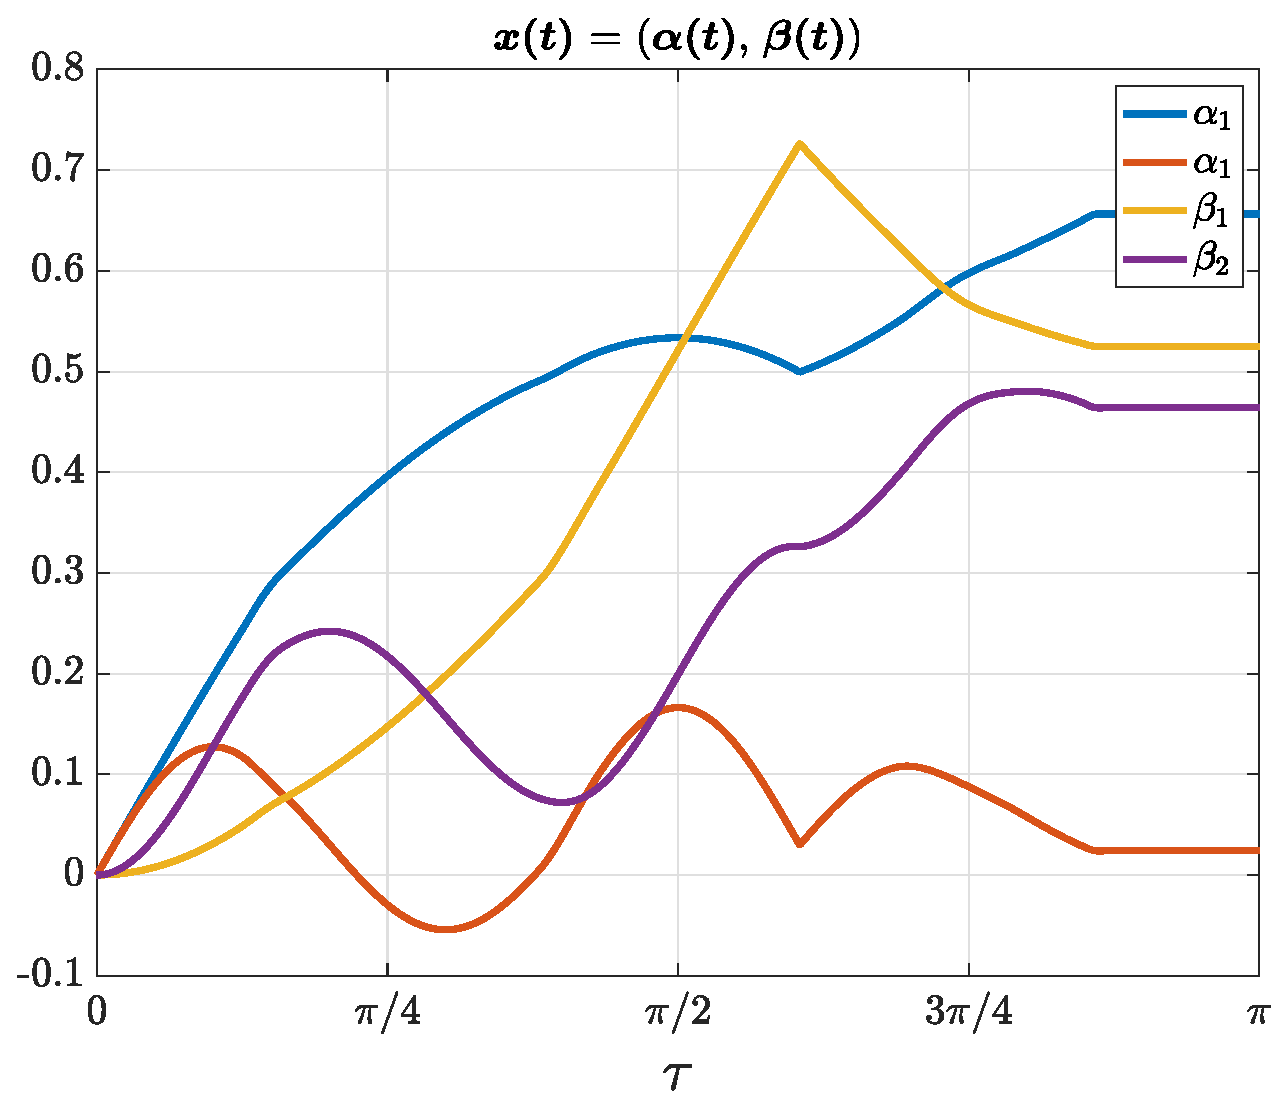
\includegraphics[scale=0.35]{img/fig02.eps}
	\caption{Evolución del sistema dinámico con los conjuntos $\mathcal{E}_a = \{1,2\}$ y $\mathcal{E}_b = \{1,2\}$ considerando el control $u(\tau)$ presentado en la figura \ref{fig:exampleSHE}}
\end{figure}

We can then formulate the following control problem, which is equivalent to Problem \ref{SHEp}:
\newline 
\begin{problem}\label{SHEpControl}
Let $\mathcal{U}$ be defined as in \eqref{eq:Udef} and let $\mathcal{E} _a $ and $\mathcal{E} _b $ be two sets of odd numbers with cardinalities $|\mathcal{E}_a| = N_a $ and $ |\mathcal{E} _b| = N_b$, respectively. Given the vectors $\bm{a}_T \in \mathbb{R}^{N_a}$ and $\bm{b}_T \in \mathbb{R}^{N_b} $, let us define $\bm{x}_T=[\bm{a}_T,\bm{b}_T]^\top \in \mathbb{R}^{N_a\times N_b}$. We look for $u:\in [0,\pi)\to\mathcal{U}$ such that the solution of \eqref{eq:CauchyReversed} with initial datum $\bm{x}(0)=\bm{x}_T$ satisfies $\bm{x}(\pi)=0$.
\end{problem}
$\newline$
\begin{remark}[Quarter-wave symmetry]
We shall mention that, in the SHE literature, it is usual to distinguish among the half-wave symmetry problem (addressed in the present paper) and the quarter-wave symmetry one in which
\begin{align*}
	u\left(\tau + \frac \pi2\right) = -u(\tau)\quad \mbox{for all}\; \tau \in \left[0,\frac \pi2\right).
\end{align*}
In quarter-wave symmetry, the SHE problem simplifies, as the Fourier coefficients $\{a_i\}_{i\in\mathcal E_a}$ turn out to be all zero. Hence, only the phases of the converter's signal can be controlled, while the half-wave SHE allows to deal with the amplitudes as well. It is worth to remark nonetheless that our optimal control formulation can be easily adapted to the quarter-wave symmetry problem by simply replacing the Fourier coefficients \eqref{eq:an} with
\begin{align*}
	a_i = 0, \quad\quad b_j = \frac{4}{\pi} \int_0^{\frac \pi4} u(\tau)  \sin(j \tau)\,d\tau.
\end{align*}
\end{remark}



\section{Optimal Control for SHE}

Since the SHE problem is equivalent to controlling a dynamic system from the origin of coordinates to a specific point, we must formulate a control problem that solves this task but also complies with the restrictions on the values that the control can take. It is necessary to set a finite subset $ \mathcal {U} $ of the interval $ [- 1,1] $, the optimal control is such that it can only take the values allowed in the discretization. In other words, the control problem is:
\begin{problem}[OCP for SHE]\label{OCP1}
    Given two sets of odd numbers $ \mathcal {E} _a $ and $ \mathcal {E} _b $ and given the target vector $ \bm {x} _T \in \mathbb {R} ^ {N_a + N_b} $, also given a set $ \mathcal {U} $ of admissible controls, we look for the function $ u (\tau) \ | \ \tau \in [0, \pi) $ such that:
    %
    \begin{gather}
        \min_{u(\tau) \in \mathcal{U}}         
         \frac{1}{2}|| \bm{x}(\pi)  ||^2   \\
        \notag \text{suject to: } \\
        \begin{cases}
            \dot{\bm{x}}(\tau) = -\bm{\mathcal{D}}(\tau) u(\tau)  & \tau \in [0,\pi)\\
            \bm{x}(0) = \bm{x}_0
        \end{cases}
    \end{gather}
\end{problem}
%
The solution of this control problem is complex due to the restriction on the admissible control values.
%
In order to obtain a problem that can be solved by classical control theory we can formulate the following control problem:

\begin{problem}[Regularized OCP for SHE]\label{OCP2}
    Given two sets of odd numbers $ \mathcal {E} _a $ and $ \mathcal {E} _b $ and given the target vector $ \bm {x} _T \in \mathbb {R} ^ {N_a + N_b} $, we look for the function $ |u (\tau)|<1 \ | \ \tau \in [0, \pi) $ such that:

    \begin{gather}
        \min_{|u(\tau) |<1}         
         \Bigg[ \frac{1}{2}|| \bm{x}(\pi)  ||^2  
        + \epsilon \int_0^{\pi} \mathcal{L}(u(\tau)) d\tau \Bigg]  \\
        \notag \text{suject to: } \\
        \begin{cases}
            \dot{\bm{x}}(\tau) = -\bm{\mathcal{D}}(\tau) u(\tau)  & \tau \in [0,\pi)\\
            \bm{x}(0) = \bm{x}_0
        \end{cases}
    \end{gather}
\end{problem}
Where we will choose $ \mathcal {L}: \mathbb {R} \rightarrow \mathbb {R} $ such that the optimal control $ u^* $ only takes values in the discretization $ \mathcal {U} $ of the interval $ [- 1.1] $. Furthermore, the parameter $ \epsilon $ should be small so that the solution minimizes the distance from the final state and the target.
%
Next we will study the optimality conditions of the problem, for a general $ \mathcal {L} $ function, and then specify how $ \mathcal {L} $ should be so that the optimal control $ u ^ * $ only takes the allowed values in $ \mathcal {U} $.

\subsection{Optimality conditions}

To write the optimility conditions of the problem we will use the principle of the Pontryagin minimum \cite[Chapter~2.7]{bryson1975applied}. For them it is necessary to define the Hamiltonian of the system, which in this case is:
\begin{gather}\label{hamil}
    H(u,\bm{p},\tau) = 
    \epsilon \mathcal{L}(u) -
    [\bm{p}^T(\tau) \cdot \bm{\mathcal{D}}(\tau)]
    u(\tau)
\end{gather}
Where the variable $ \bm{p} (\tau) $ called adjoint state is introduced, which is associated with the restriction imposed by the system. Este tiene la misma dimensión del estado, de manera que 
\begin{gather}
        \bm{x}(\tau) = \begin{bmatrix}
            \bm{\alpha}(\tau) \\  \bm{\beta}(\tau)
        \end{bmatrix}   \Leftrightarrow
        \bm{p}(\tau) = \begin{bmatrix}
        \bm{p}^\alpha(\tau) \\ \bm{p}^\beta(\tau)
                \end{bmatrix}
\end{gather}
A continuación enumeraremos las condiciones de optimalidad provenientes del prinicio de mínimo de Pontryagin.

\begin{enumerate}

    \item \textbf{Final condition of the adjoint}: This optimiality condition is obtained from the cost in the final time $\tau = \pi$ of the control problem in this case $ \Psi (\bm{x}) = \frac {1}{2} \| \bm{x} (\pi) - \bm{x}_T \|^2 $.
    \begin{gather}
        \bm{p}(\pi) = \nabla_{\bm{x}} \Psi(\bm{x}) =  (\bm{x} (\pi) - \bm{x}_T)
    \end{gather}
    %%%%%%%%%%%%%%%%%%%%%%%%%%%%%%%%%%%%%%%%%%
    \item \textbf{Adjoint evolution equation}: 
    \begin{gather}
        \dot{\bm{p}}(\tau) = -\nabla_x H(u(\tau),\bm{p}(\tau),\tau) = 0
    \end{gather}
    From where it can be deduced that $ \bm {p} (\tau)$ is a constant so that $ \bm {p} (\tau) = \bm {x} (\pi) - \bm { x} _T \ | \ \forall \tau \in [0, \pi) $ so from now on we will refer to it simply as $ \bm {p} $, noting that it is invariant in time.
    \item \textbf{Optimal control shape}: We known that $ u^* = \argmin_{|u|<1} H(\tau,\bm{p}^*,u)$, so in this case we can write:
    \begin{gather}
        u^*(\tau) = \argmin_{|u|<1}  \Big[   \epsilon \mathcal{L}(u(\tau)) -
        [{\bm{p}^*}^T \cdot \bm{\mathcal{D}}(\tau)]
        u(\tau) \Big]
    \end{gather}
    Therefore, this optimality condition reduces to the optimization of a function in a variable within the interval $ [- 1,1] $. 
\end{enumerate}
%
Es importante recordar que 
    \begin{gather}
        [{\bm{p}^*}^T \cdot \bm{\mathcal{D}}(\tau)] = \sum_{i \in \mathcal{E}_a} p^*_\alpha \cos(i\tau) + \sum_{j \in \mathcal{E}_b} p^*_\beta \sin(j\tau) \ | \ \forall \tau \in [0,\pi)
    \end{gather}
we build a function $\mathcal{H}_m: [-1,1] \rightarrow \mathbb{R}$ such that:
\begin{gather}
    \mathcal{H}_m(u) = \epsilon \mathcal{L}(u) - mu  |  \forall m \in \mathbb{R}
\end{gather}
Donde hemos remplazado el término $[{\bm{p}^*}^T \cdot \bm{\mathcal{D}}(\tau)]$ por un parámetro $m$ que puede variar en todo la recta real. Es decir, el problema para diseñar un problema de control óptimo que solo pueda tomar valores en $\mathcal{U}$ se reduce a diseñar una función unidimensional  com parámertro $m$ cuyos mínimos sean los elementos de $\mathcal{U}$ para cualquier valor de $m$. 
\subsection{Piecewise linear penalization}

En esta subsección presentaremos como diseñar el término de penalización $\mathcal{L}(u)$ para que el control óptimo en cualquier caso este contenida en $\mathcal{U}$. 
% \begin{proposition}
%     Consideremos que tenemos un conjunto de elementos $\mathcal{U} = \{u_1,u_2,\dots,u_{N_u}\}$, además consideraremos una función de penalización $\mathcal{L}(u)$ que define la función $\mathcal{H}_m(u)$. Entonces si los puntos $\{u_k,\mathcal{L}(u_k)\}_{k=1}^{N_u}$ son la envolvente convexa de ellos mismos entonces los mínimos de $\mathcal{H}_m(u)$ son los elementos de $\mathcal{U}$.
% \end{proposition}
%
De manera más concreta podemos elegir la interpolación afín de una parábola  $\mathcal{L}:[-1,1] \rightarrow \mathbb{R}$ como término de penalización. Es decir:  
\begin{gather}\label{PLP}
    {\mathcal{L}(u)} = \begin{cases}
        \big[ (u_{k+1}+u_{k}) (u-u_k) + u_k^2 \big] & \text{if}  u \in [u_k,u_{k+1}[ \\
        1 & \text{if} \ u = u_{N_u} 
    \end{cases} \\
    \notag \forall k \in \{1,\dots,N_u-1\}
\end{gather}
%
Entonces el Hamiltoniano queda como:
\begin{gather}
    {\mathcal{H}_m(u)} = \begin{cases}
        \epsilon\big[ (u_{k+1}+u_{k}) (u-u_k) + u_k^2 \big] -mu & \text{if}  u \in [u_k,u_{k+1}[ \\
        \epsilon-mu & \text{if} \ u = u_{N_u} 
    \end{cases} \\
    \notag \forall k \in \{1,\dots,N_u-1\}
\end{gather}


%
De manera que para calcular el mínimo de $\mathcal{H}_m(u)$ deberemos considerar que esta función no es diferenciable por lo que la condicion de optimizalidad no puede realizarse con la difereciación típica sino con la subdiferencial.

Entonces calulremos la subdiferecial $\partial \mathcal{H}_m$ todo 
\begin{gather}
    \partial \mathcal{H}_m(u) = \begin{cases}
         \{\epsilon(u_1 + u_2) - m \}   & \text{if} \ u = u_1 \\
         %%%%%%%%%%%%%%%%%%%%%%%%%%%%%%%%%%%%%%%%%%%%%%%%
         \{\epsilon(u_k + u_{k+1})-m\}  & \text{if} \ u \in \ ]u_k,u_{k+1}[ \hspace{1.1em} \dagger\\
         %%%%%%%%%%%%%%%%%%%%%%%%%%%%%%%%%%%%%%%%%%%%%%%%
         [\epsilon(u_k+u_{k-1})-m \ , \ \epsilon(u_{k+1}+u_k)-m] & \text{if} \ u = u_k \hspace{4.em} \dagger \dagger \\
         %%%%%%%%%%%%%%%%%%%%%%%%%%%%%%%%%%%%%%%%%%%%%%%%%
         \{\epsilon(u_{N_u} + u_{N_u-1}) - m \} & \text{if} \ u = u_{N_u} 
    \end{cases} \\
    \notag \dagger \ \forall k \in \{1,\dots,N_u-1\} \hspace{4em}
    \dagger \dagger \ \forall k \in \{2,\dots,N_u-1\}
\end{gather} 

Entonces dado $m\in \mathbb{R}$ busamos $u \in [-1,1]$ que minimiza $\mathcal{H}_m(u)$. Es necesario comprobar que cero perteneca al subdiferecial $\partial \mathcal{H}_m(u)$

\begin{itemize}
    \item \textbf{Case 1: $m \leq \epsilon(u_1+u_2)$}: Dado que $m$ es menor que el menor de todos los subdiferenciales entonces el cero no se encuentra dentro de ninguna de los intervalos definidos para la subdiferencial. De manera que el mínimo esta en un extremo
    \begin{gather}
        \argmin_{|u| < 1} \mathcal{H}_m(u) = u_1
    \end{gather} 
    \item \textbf{Case 2: $m = \epsilon(u_{k+1}+u_k) $}:  Teniendo en cuenta que $\forall k \in \{1,\dots,N_u-1\}$.
    \begin{gather}
        \argmin_{|u| < 1} \mathcal{H}_m(u) = [u_k,u_{k+1}[ 
    \end{gather} 
    \item \textbf{Case 3: $\epsilon(u_k+u_{k-1})<m<\epsilon(u_{k+1}+u_k)$} : Teniendo en cuenta que $\forall k \in \{2,\dots,N_u-1\}$.
    \begin{gather}
        \argmin_{|u| < 1} \mathcal{H}_m(u) = u_k
    \end{gather}
    \item \textbf{Case 4: $m>\epsilon(u_{N_u}+u_{N_u-1})$}:
    \begin{gather}
        \argmin_{|u| < 1} \mathcal{H}_m(u) = u_{N_u}
    \end{gather} 
\end{itemize}

Es decir solo cuando  $m = \epsilon(u_{k+1}+u_k)$ los mínimos del Hamiltoniano esta dentro de un intervalo, para otros valores de $m$ los mínimos del Hamiltoniano están contenidos en $\mathcal{U}$. Así que ante una variación continua de $m$ el caso 2 solo ocurrirá de manera puntal. Recordando en el problema de control óptimo $m(\tau) = [\bm{p}^T(\tau) \cdot \bm{\mathcal{D}}(\tau)]$, podemos notar que el caso 2 corresponde a los instantes $\tau$ de cambio de valor.
\section{Numerical simulations}\label{Section5}

In this section, we will present several examples in which we solve our optimal control problem through the direct method and the non-linear constrained optimization tool \texttt{CasADi} \cite{Andersson2019}.
%
\subsection{Smooth approximation of piece-wise linear penalization}

With the final aim of using an optimization software to solve our optimal control problem, we will approximate our piece-wise linear penalization with the help of the Heaviside function $h:\mathbb{R} \rightarrow \mathbb{R}$ and its smooth approximation defined as follows: 
\begin{gather}
    h(x) = \begin{cases}
        1 & \text{ if } x \geq 0 \\
        0 & \text{ if } x < 0
    \end{cases}    
    \hspace{2em} 
    \begin{cases}
        h^\eta(x) = (1 + \tanh(\eta x))/2   \\
        \eta \rightarrow \infty
    \end{cases}
\end{gather}
Using $h$, we can define the (smooth) function $\Pi_{a,b}^\eta:\mathbb{R} \rightarrow \mathbb{R}$ as:
\begin{align*}
    \Pi_{[a,b]}^\eta(x) &= - 1 + h^\eta(x-a) + h^\eta(-x+b) 
    \\
    &= \frac{\tanh[\eta( x -a)] + \tanh[\eta (b-x)]}{2}.
\end{align*}
In this way, we can define the smooth version of \eqref{PLP}:
\begin{gather}
    \mathcal{L}^\eta(u) = \sum_{k = 1}^{N_u-1} \big[ (u_{k+1}+u_{k}) (u-u_k) + u_k^2 \big] \Pi^\eta_{[u_k,u_{k+1}]}(u)
\end{gather}
So that, when $\eta \rightarrow \infty$, then $\mathcal{L}^\eta \rightarrow \mathcal{L}$.

\subsection{Direct method  for  OCP-SHE}

To solve the optimal control problem (\ref{OCP2}), we use a direct method. 
%
If we consider a partition $\mathcal{P} = \{\tau_0,\tau_1,\dots,\tau_{T}\}$ of interval $[0,T]$ , we can represent a function $\{ u(\tau) \ | \ \tau \in [0,T]\}$ as a vector $\bm{u} \in \mathbb{R}^{T}$ where component $u_t = u(\tau_t)$. 
%
Then the optimal control problem (\ref{OCP1}) can be written as optimization problem with variable $\bm{u} \in \mathbb{R}^{T}$. This problem is a nonlinear programming, for this we use CasADi software to solve. 
%
Hence, given a partition of the interval $[0,\pi)$, we can formulate the problem \eqref{OCP1} as the following one in discrete time

\begin{problem}[Numerical OCP]
Given two sets of odd numbers $\mathcal{E}_a$ and $\mathcal{E}_b$ with cardinalities $|\mathcal{E}_a| = N_a$ and $|\mathcal{E}_b| = N_b$ respectively, given the target vectors $\bm{a}_T  \in \mathbb{R}^{N_a}$, so that $\bm{x}_0 = [\bm{a}_T,\bm{b}_T]^T$ and $\bm{b}_T \in \mathbb{R}^{N_b}$ and a partition $\mathcal{P}_\tau = \{\tau_0,\tau_1,\dots,\tau_{T}\}$ of the interval $[0,\pi)$, we search a vector $\bm{u} \in \mathbb{R}^{T}$ that minimizes the following function:
\begin{gather}
        \min_{\bm{u} \in \mathbb{R}^{T} } 
        \Bigg[ 
        || \bm{x}^{T}||^2
        + \epsilon  \sum_{t=0}^{T-1} \mathcal{L}^\eta(u_{t}) \Delta\tau_t  \Bigg]  \\
        \notag \text{suject to: } \\
        \forall \tau \in \mathcal{P} \begin{cases}
            \bm{x}^{t+1} = \bm{x}^{t} - (2/\pi)\Delta \tau_t \bm{\mathcal{D}}(\tau_t)u_t \\
            \bm{x}^0 = \bm{x}_0
        \end{cases} 
\end{gather}
\end{problem}

\subsection{Resultados}

All our simulations have been performed with a laptop with $8Gb$ of RAM memory and the execution time for finding the solution given a target vector is os the order of $1s$. IN what follows, we will discuss all the numerical results we have obtained
\begin{enumerate}    
    \item \textbf{OCP with quarter-wave symmetry}: we will consider the problem with a set of odd numbers $\mathcal{E}_b = \{1,5\}$ and a discretization of $[0,\pi/2]$ with $T = 200$. We show the solutions for the target vectors $b_T^1 = \{(-0.4,-0.3,\dots,0.3,0.4)\}$ keeping $b_T^5=0$ for each case. We display the optimal trajectories we obtained in Figure \ref{ex01}, where we can see a continuity of the solutions with respect to the target vector.

    % \begin{figure}
    %     \centering
    %     \begin{subfigure}[b]{\textwidth}
    %         \centering
    %         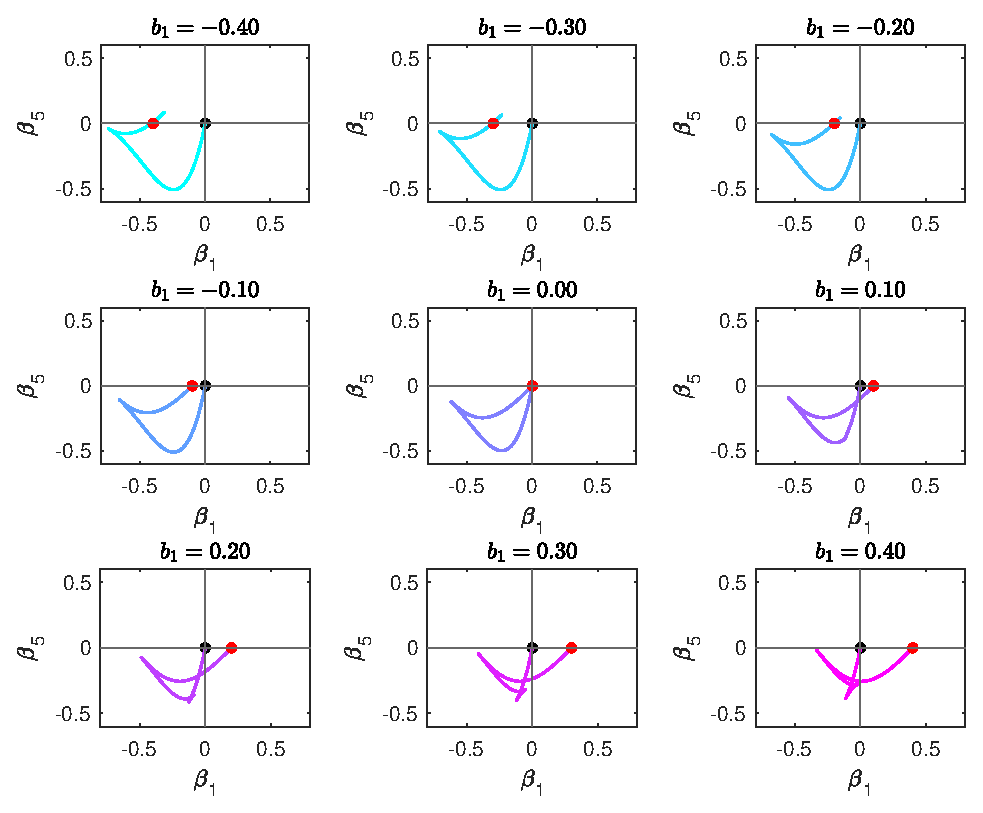
\includegraphics[width=0.6\textwidth]{img/ex01-con.eps}
    %         \caption{Dynamical System: el punto rojo hace referencia al punto final mientras que el punto negro hace referencia al punto inicial.}
    %     \end{subfigure} 
    %     \hfill \\
    %     \begin{subfigure}[b]{\textwidth}
    %         \centering
    %         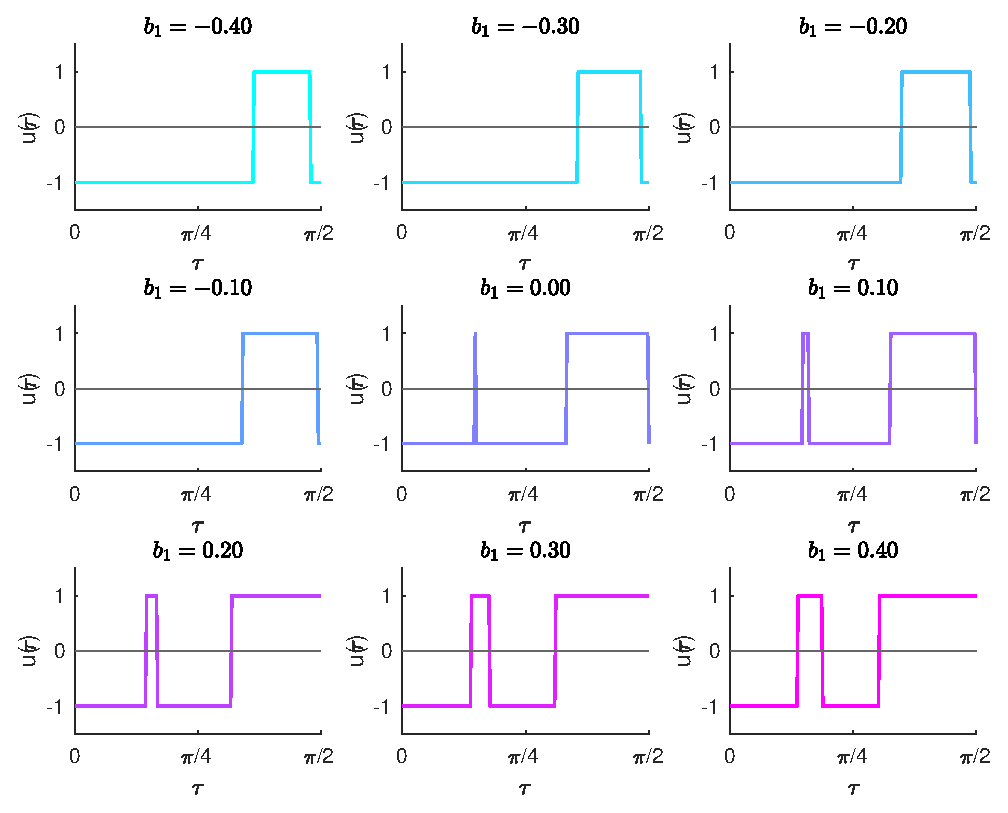
\includegraphics[width=0.6\textwidth]{img/ex01-dyn.eps} 
    %         \caption{Control}
    %     \end{subfigure}
    %     \caption{Mostramos las trayectorias óptimas y controles óptimos para distintos vectores objetivo.}
    %     \label{ex01}
    % \end{figure}


    \item \textbf{OCP with quarter-wave symmetry for an interval of $b_1$}: for this example we consider the following set of odd numbers: $\mathcal{E}_b = \{1,5,7,11,13\}$. 
    %
    Moreover, we consider the target vector $\bm{b}_T = [m_a,0,0,0,0]$, where $m_a \in [-1,1]$ is a parameter, with three penalization terms: $\mathcal{L}(u) = -f$, $\mathcal{L}(u) = +f$ and $\mathcal{L}(u) = -f^2$ obtained by direct method with uniform partition of interval $[0,\pi/2]$ with $T=400$ and penalization parameter $\epsilon = 10^{-5}$. 
    %
    For each one of the penalization terms we will employ, the distance between the Fourier coefficients is of the order $10^{-4}$. 
    %
    Nevertheless, when the penalization term is $\mathcal{L}(u)= -f^2$, the solution does not present continuity with respect to the target vector. 
    %
    On the other hand, it is important to mention that the solutions for the penalization terms $\mathcal{L}(u) = -f$ y $\mathcal{L}(u) = f$ are symmetric, so that inverting those solutions with respect to the origin and inverting their sign, it can be observed that they are the same.
     
    \item \textbf{SHE with three levels}: we can see that in the case in which the control $u(\tau)$ can only take values in $[0,1]$, we obtain signals which can take three levels in the interval $[0,2\pi]$ due to the quarter-wave symmetry. If we solve the optimal control problem this time with restrictions $\{0<u(\tau)<1\}$. We repeat the same procedure as before, thus obtaining solutions for the same penalization terms and obtaining Figure \ref{ex3LVL}. There we show the continuity of the solutions and that they are of the order $10^{-4}$.
    



    
      


    \item \textbf{Changes in the commutations number}: thanks to the optimal control formulation of SHE, we can vary the number of commutation angles. 
    %
    This is illustrated in the following example, where we considered the set of odd numbers $\mathcal{E}_b = \{1,3,9,13,17\}$. Moreover, we consider the target vector $\bm{b}_T = [m_a,0,0,0,0]$, where $m_a \in [0,1]$ is a parameter. 
    %
    In this problem, we used the penalization $\mathcal{L} = f$ with a penalization parameter $\epsilon=10^{-4}$.
    %
    We can see in Figure \ref{disco} that the optimal control problem is capable of moving among different solution sets.




    
    \item \textbf{OCP for SHE with half-wave symmetry}: we considered the optimal control problem in half-wave with $\mathcal{E}_a = \{1,3,5\}$ and  $\mathcal{E}_b = \{1,3,5,9\}$, where $\bm{a}_T = [m_a,0,0]$, $\bm{b}_T = [m_a,m_a,0,0]$ and $m_a \in [-0.6,0.6]$. We chose the penalization $L(u) = +f$



\end{enumerate}







\section{Conclusiones}\label{Section6}


Se ha presentado el problema SHE desde un punto de vista de la teoría de control. Esta metodología es efectiva para llega a presiciones $10^{-4}-10^{-5}$ en la distancia al vector objetivo. Sin embargo en comparación con metodologías donde el número de conmutaciones es prefijado, nuestra aproximación es más costosa. Sin enbargo, el control óptimo asegura soluciones en todo el rango de indice de modulación, aunque el número de soluciones o la localización de estas cambien abruptamente.

Este plantamiento del problema SHE enlaza la teoría de control con la eliminación de harmónicos. De esta manera el problema SHE se puede resolver mediante herramientras clásicas.

\begin{ack}                               % Place acknowledgements
Partially supported by the Roman Senate.  % here.
\end{ack}
 
\bibliographystyle{apalike}        % Include this if you use bibtex 
\bibliography{bib}           % and a bib file to produce the 
                                 % bibliography (preferred). The
                                 % correct style is generated by
                                 % Elsevier at the time of printing.




\end{document}